\documentclass{beamer}
 
\usepackage[utf8]{inputenc}
 
 
%Information to be included in the title page:
\title[BSD]{Verifying some consequences of the Birch Swinnerton-Dyer Conjecture}
\author{Felipe Jacob}
\institute[UCL]{University College London}
\date{2017}
 
\begin{document}

\newcommand{\defin}{\textbf}
\newcommand{\CC}{{\mathbb C}}
\newcommand{\cov}{{\operatorname{cov}}}
\newcommand{\eE}{{\mathcal E}}
\newcommand{\NN}{{\mathbb N}}
\newcommand{\PP}{{\mathbb P}}
\newcommand{\ZZ}{{\mathbb Z}}
\renewcommand{\SS}{{\mathbb S}}
\newcommand{\DD}{{\mathbb D}}
\newcommand{\RR}{{\mathbb R}}
\newcommand{\QQ}{{\mathbb Q}}
\newcommand{\rR}{{\mathcal R}}
\newcommand{\OO}{{\mathcal O}}
\newcommand{\p}{\partial}
\newcommand{\mM}{{\mathcal M}}
\newcommand{\pP}{{\mathcal P}}
\newcommand{\iI}{{\mathcal I}}
\newcommand{\jJ}{{\mathcal J}}
\newcommand{\uU}{{\mathcal U}}
\newcommand{\sS}{{\mathfrak S}}
\newcommand{\1}{{\mathds 1}}
\newcommand{\Crit}{\operatorname{Crit}}
\newcommand{\GKK}{{G_{\bar{K} : K}}}
\newcommand{\st}{{\text{s.t.}}}
\newcommand{\ra}{\rightarrow}
\newcommand{\Sel}{\text{\normalfont Sel}}
\newcommand{\Sha}{\text{\normalfont Sha}}
\newcommand{\TS}{\text{\normalfont TS}}
\newcommand{\Eb}{\bar{E}}
\newcommand{\EQ}{E(\QQ)}
\newcommand{\cmark}{\textrm{\ding{51}}}
\newcommand{\xmark}{\textrm{\ding{55}}}
\newcommand{\EFp}{{\tilde{E}(\FF_p)}}
\newcommand{\EFt}{{\tilde{E}(\FF_2)}}
\newcommand{\EQp}{{E(\QQ_p)}}
\newcommand{\FF}{\mathbb{F}}
\newcommand{\HH}{\mathbb{H}}
\newcommand{\Tors}{{\text{\normalfont Tors}}}
\newcommand{\parder}[2]{\frac{\partial #1}{\partial #2}}
\newcommand{\Zpx}{\mathbb{Z}_p^\times}
\newcommand{\legendre}[2]{\left(\frac{#1}{#2}\right)}
\newcommand{\quadring}[1]{\ZZ[\sqrt{#1}]}
\newcommand{\Ip}{\mathfrak{p}}
\newcommand{\Aa}{\mathbb{A}}
\newcommand{\LL}{\mathcal{L}}
\newcommand{\Shim}{\textnormal{Shim}}

\frame{\titlepage}
 
\begin{frame}
\frametitle{Elliptic Curves}
In this project we will be considering the arithmetic properties of
\textbf{elliptic curves} $E(K)$. These are given by the set of points $(x, y)$
with $x$ and $y$ in
the field $K$ such that
\[E: y^2 = f(x),\]
where $f(x)$ is a cubic polynomial with 3 distint roots.
\end{frame}

\begin{frame}
\frametitle{Elliptic Curves}
  We always assume that we have a known point $\OO \in E(K)$ in the projective
  completion $\PP^2(K)$, which is called the \textbf{point at infinity of $E$}. \pause

  When $K$ doesn't have characteristic 2, we can assume that the curve is given
  by the equation
  \[y^2 = x^3 + ax^2 + bx + c,\]
  with $a, b, c \in K$, and that $\OO = (0:1:0).$
\end{frame}

\begin{frame}
  \frametitle{Group Law}
  Elliptic curves are interesting because on top of being a variety, they also
  form an abelian group. To add two distinct points $P, Q$, we trace the line
  between them and let $R$ be the third point of intersection of this line with
  the curve. $P+Q$ is then the reflection of $R$ over the $x$-axis. \pause
  \begin{figure}
    \centering
  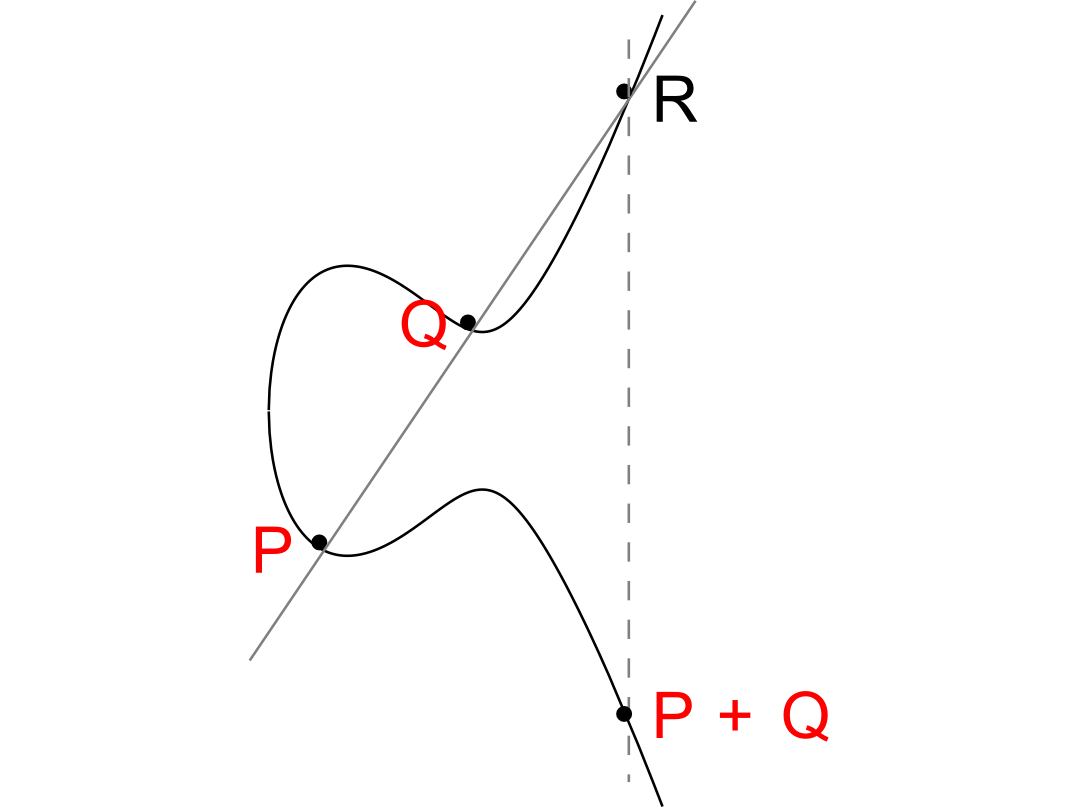
\includegraphics{picture3}
  \end{figure} \pause

  Under this addition, it turns out that $E(K)$ is an abelian group.
\end{frame}

\begin{frame}
  \frametitle{Quadratic Twists}
  The curves we will be interested in this project are given by
  \[E_n : y^2 = x^3 - n^2 x,\]
  where $n$ is odd and squarefree. \pause

  They are notorious for their relation with Fermat and the
  congruent number problem.
\end{frame}

\begin{frame}
  \frametitle{The Rank}
  The Mordell-Weil Theorem states that when $K = \QQ$, the group $E(\QQ)$ is
  finitely generated. This means that we can write
  \[E(\QQ) \simeq \Tors(E(\QQ)) \times \ZZ^r,\]
  where $\Tors(E(\QQ))$ are the points of finite order, and $r$ is a natural
  number, called the \textbf{rank of $E$}. \pause
  \bigskip

  Computing $\Tors(E(\QQ))$ is easy, but finding $r$ for arbitrary
  curves is very much an open problem. In this presentation we will discuss a
  few techniques used in such computations.
\end{frame}
 
\begin{frame}
  \frametitle{The BSD Conjecture}
  The Birch Swinnerton-Dyer Conjecture relates the rank $r$ of an elliptic
  curve $E$ to the order of a zero of a certain analytic function. \pause

  More precisely, it says that
  \[L(E,s) = C (s-1)^r + O((s-1)^{r+1}),\]
  where $L(E,s)$ is an analytic function called the \textbf{Hasse-Weil
    L-function of $E$}. We will see how to construct it.
\end{frame}
 
\begin{frame}
  \frametitle{Local Zeta Functions}
  Let $p$ be a prime number.
  If $V$ is a variety over $\FF_p$, we can construct the \textbf{Local Zeta
    Functions of $V$ at $p$}, given by
  \[Z(V,p,s) = \exp \left( \sum\limits_{k=1}^\infty \# V(\FF_{p^k})
      \frac{z^k}{k} \right).\] \pause
  These capture the behaviour of $V$ in all finite fields of $p^k$ elements.
\end{frame}

\begin{frame}
  \frametitle{Local Zeta Functions}
  As an example, if $V$ is a point, then $\# V(\FF_{p^k}) = 1$, so we get
  \begin{equation*}
    \begin{split}
      Z(V,p,s) &= \exp \left( \sum\limits_{k=1}^\infty \frac{z^k}{k} \right)
      = \exp \left( -\log (1-z) \right) \\
      &= \frac{1}{1-z}
    \end{split}
  \end{equation*} \pause

  Similarly, if $V = \PP^n$, we know that $\# V(\FF_{p^k}) = 1 + p^k + \cdots +
  p^{nk}$, so we get 
  \[Z(V,p,z) = \frac{1}{1-z} \frac{1}{1-pz}\cdots \frac{1}{1-p^nz}\]
\end{frame} 

\begin{frame}
  \frametitle{Hasse-Weil L-Function}
  To form the \textbf{Hasse-Weil L-function of $V$},
  we multiply the local zeta functions
  of $V$ for all different primes:

  \[L(V,s) = \prod\limits_p Z(V,p,p^{-s}).\] \pause

  This function captures the behaviour of $V$ at all possible finite fields.

\end{frame}

\begin{frame}
  \frametitle{Hasse-Weil L-function}
  For the case where $V$ is a point, we get
  \[L(V,s) = \prod \limits_p \frac{1}{1-p^{-s}} = \zeta(s)\]
  which is the classical Riemann-Zeta function. \pause 

  If $V = \PP^n$ we instead get
  \[L(V,s) = \zeta(s) \zeta(s-1) \cdots \zeta (s-n).\]
\end{frame}

\begin{frame}
  \frametitle{Hasse-Weil L-function}
  For the family of elliptic curves $E_n$, the Hasse-Weil L-function takes the
  form
  \[L(E_n, s) = \prod\limits_{p \nmid 2n} \frac{1}{1 - 2a_{n,p}p^{-s} + p^{1-2s}},\]
  where the $a_{n,p}$ are certain integers depending on $n$ and $p$.
\end{frame}

\begin{frame}
  \frametitle{Full BSD}
  The full BSD conjecture also relates the constant $C$ in the prediction
  \[L(E,s) = C(s-1)^r + O((s-1)^{r+1})\]
  to certain arithmetic invariants of $E$. \pause
  \bigskip

  In particular, it states that
  \[C = \frac{\# \Sha(E) R_E \Omega_E}{\# \Tors(E)^2} \prod\limits_p c_p\]
  where we will define each of these quantities.
\end{frame}

\begin{frame}
  \frametitle{Tate-Shafarevich Group}
  The group $\Sha(E)$ is called the \textbf{Tate-Shafarevich group of $E$}. It
  is an abelian group, conjectured to be finite, and measures in some sense how
  hard it is to find the rank by local methods. \pause
  \bigskip
  
  The full definition requires the machinery of Galois Cohomology, and takes the
  form
  \[\Sha(E) = \textnormal{Ker} \left( H^1(\QQ,\bar{E}) \ra \prod\limits_\nu
    H^1(\QQ_\nu, \bar{E})\right).\]
\end{frame}

\begin{frame}
  \frametitle{Regulator}
  The \textbf{regulator of $E$} measures in a specific sense the volume of a set
  of generators of $E$. \pause
  \bigskip

  It is defined by
  \[R_E = \det \left( \langle P_i, P_j \rangle \right)\]
  where $P_1, \dots, P_r$ is a basis for $\frac{E(\QQ)}{\Tors(E(\QQ))}$ and
  $\langle \cdot \rangle$ is an inner product on $E(\QQ)$ called the Neron-Tate pairing.
\end{frame}

\begin{frame}
  \frametitle{Real Period}
  The \textbf{real period of $E$} is given by the line integral
  \[\Omega_E = \int_{E(\RR)} \frac{dx}{2y}.\]

  For the curves $E_n$, we have
  \[\Omega_{E_n} = \frac{2}{\sqrt{n}} \beta,\]
  where $\beta = \int_1^\infty \frac{dx}{\sqrt{x^3-x}} \approx 2.622.$
\end{frame}

\begin{frame}
  \frametitle{Tamagawa Numbers}
  The \textbf{Tamagawa Numbers $c_p(E)$} capture the behaviour of $E$ at the
  primes where it has bad reduction. If $E$ is given by
  \[E: y^2 = f(x)\]
  and the polynomial $f(x)$ still has 3 distinct roots in $\FF_p$, we say that
  $E$ has good reduction at $p$. In this case there is a homomorphism of curves
  \[E(\QQ) \ra E(\FF_p)\]
  given by reduction modulo $p$.
\end{frame}

\begin{frame}
  \frametitle{Tamagawa Numbers}
  If $\Delta(f) \equiv 0 \, (p)$, the reduction map may no longer be a
  homomorphism. The situation
  can still be salvaged, however. \pause
  \bigskip

  Let $E(\FF_p)_{ns}$ be the set of points $(x,y)$ where $E(\FF_p)$ is
  nonsingular. Looking at the completion $\QQ_p$ we still have a map
  \[E(\QQ_p) \ra E(\FF_p).\] \pause
  If we let $E(\QQ_p)_0$ be the preimages of the nonsingular points, then the
  restriction
  \[E(\QQ_p)_0 \ra E(\FF_p)_{ns}\]
  is still a homomorphism.
\end{frame}

\begin{frame}
  \frametitle{Tamagawa Numbers}
  The Tamagawa Numbers $c_p$ of $E$ are defined by
  \[c_p = \left| \frac{E(\QQ_p)}{E(\QQ_p)_0} \right|.\]
  They measure the number of singular components of $E$. This is usually a power
  of 2.\pause
  \bigskip

  \begin{theorem}
    In the project, we calculated that for $n$ odd and squarefree, we have
    \[\prod\limits_p c_p(E_n) = 2 \cdot 4^{\omega(n)},\]
    where $\omega(n)$ is the number of distinct prime factors of $n$.
  \end{theorem}

\end{frame}

\begin{frame}
  \frametitle{The situation so far}
  From the information we currently have, the situation seems pretty hopeless.
  On the one hand we have $L(E_n,s)$ given by a complicated product. On the
  other we have a constant $C$ that involves the transcendental number $\beta$
  and lots invariants of $E_n$. \pause
  \bigskip
  
  The way forward is given by \textbf{Tunnell's Theorem}, a very deep result
  coming from the theory of Modular Forms, and which will allow us to compute
  $L(E_n,s)$ more explicitly.
\end{frame}

\begin{frame}
  \frametitle{Tunnell's Theorem}
  Let $\Theta(z) = \sum\limits_{m \in \ZZ} q^{m^2}$ where $q = e^{2 \pi i z}$ be
  the Theta function. \pause
  \begin{theorem}[Tunnell's Theorem]
    For $n$ odd, the critical values $L(E_n,1)$ are given by
    \[L(E_n,1) = \frac{\beta}{4\sqrt{n}} a_n^2.\]
    Here $a_n$ are the Fourier coefficents of the function
    \[f(z) = \sum\limits_{m \in \ZZ} a_m q^m = \Theta(z) \left( \Theta(32z)
      - \frac{1}{2}\Theta(8z)\right) \Theta(2z)\]
  \end{theorem}
\end{frame}

\begin{frame}
  \frametitle{BSD Revisited}
  Here we are lucky to have the same $\beta$ occuring on both sides of the BSD
  conjecture: 

  \[L(s,1) = \frac{\# \Sha(E_n) R_{E_n} \Omega_{E_n}}{\#\Tors(E(\QQ))^2}\] 
  becomes, at $s = 1$: \pause
  \[\frac{\beta}{4 \sqrt{n}} a_n^2 = \frac{\# \Sha(E_n) R_{E_n} 2 \beta}{
      16 \sqrt{n}} \cdot 2 \cdot 4^{\omega(n)} \cdot 0^r,\] \pause
  which simplifies to
  \[a_n^2 = \# \Sha(E_n) \cdot R_{E_n} \cdot 4^{\omega(n)} \cdot 0^r.\]

\end{frame}

\begin{frame}
  \frametitle{BSD Revisited}
  We have
  \[a_n^2 = \# \Sha(E_n) \cdot R_{E_n} \cdot 4^{\omega(n)} \cdot 0^r.\]
  Since when the rank is nonzero, the BSD conjecture says nothing interesting
  about the right hand side, we will assume $r = 0$. In this case $R_{E_n} = 1,$
  so this further simplifies to
  \[a_n^2 = 4^{\omega(n)} \# \Sha(E_n).\] \pause

  This is now an equation of \textbf{integers}, so we can hope to use some
  number theory to show it is true. In the project we were able to prove that it
  indeed holds at least modulo 16.
\end{frame}

\begin{frame}
  \frametitle{Outline of Calculations}
  In order to verify that
  \begin{equation} \label{eq:mainpred}
    a_n^2 \equiv 4^{\omega(n)} \# \Sha(E_n) \mod{16}
  \end{equation}
  we
  \begin{itemize}
  \item Worked out the coefficients $a_n$ modulo 4. This turns out to
    depend on $n$ modulo 8.
  \item Found the Selmer Group of $E_n$, a computable complement of
    $\Sha(E_n).$ This also depends on $n$ modulo 8.
  \item Matched both informations with Equation \autoref{eq:mainpred}
    for each residue class
    of $n$ modulo 8.
  \end{itemize}
\end{frame}

\begin{frame}
  \frametitle{Calculation of Coefficients of Theta Series}
  Recall that we want to compute the integers $a_m$ modulo 4, where
    \[f(z) = \sum\limits_{m \in \ZZ} a_m q^m = \Theta(z) \left( \Theta(32z)
      - \frac{1}{2}\Theta(8z)\right) \Theta(2z).\] \pause

  But this is equivalent to 
  \[f(z) = \sum\limits_{x,y,z \in \ZZ} q^{2x^2 + y^2 + 32z^2} - \frac{1}{2}
  \sum\limits_{x,y,z \in \ZZ} q^{2x^2 + y^2 + 8z^2}.\] 
\end{frame}

\begin{frame}
  \frametitle{Calculation of Coefficients of Theta Series}
  In other words, we want to know among the solutions to
  \[2x^2 + y^2 + 8z^2 = n\]
  how many are also solutions to
  \[2x^2 + y^2 + 32z^2 = n. \] 
  Since we only want this mod 4, we can use many tricks.
\end{frame}

\begin{frame}
  \frametitle{Calculation of Selmer Group}
  To calculate the Selmer group, we saw in MATH3703 that we have to solve a
  bunch of equations of the form
  \[N^2 = d_1M^4 + \frac{4n^2}{d_1} e^4\]
  in $\QQ_p$ for each prime $p.$ \pause
  \bigskip

  This can be done by some extensive applications
  of quadratic reciprocity together
  with Hensel's lemma.
\end{frame}

\begin{frame}
  \frametitle{Conclusion}
  From our calculations we deduced that if $p$ is an odd prime,
  \[a_p \equiv
    \begin{cases}
      0 \mod{4} \quad &\text{if } p \equiv 1,5,7 \mod{8} \\
      2 \mod{4} \quad &\text{if } p \equiv 3 \mod{8}
    \end{cases}
  \]
  and $a_n \equiv 0 \, (4)$ if $n$ is composite. \pause
  \bigskip

  We also found that $\Sha(E_p)$ has an element of 2-torsion if and only if $p
  \not\equiv 3 \, (8).$ \pause
  \bigskip

  Putting both results together gives
  \[a_n^2 \equiv 4^{\omega(n)} \# \Sha(E_n) \mod{16},\]
  verifying the Birch Swinnerton-Dyer conjecture modulo 16, as wanted.
\end{frame}

\end{document}
